\section{Practical}
	\subsection{Creating the The App}
	CI/CD was demonstrated using a simple web app. The objective was to create a web app which can be continuously deployed to AWS. For demonstration purposes a very basic app was created using NodeJS library ReactJS. It is simply a frontend web app that displays a basic ReactJS homepage as a visual indication of a successful deploy. The app running locally can be seen in \autoref{fig:app-local}.
	\begin{figure}[H]
		\caption{React App}
		\centering
		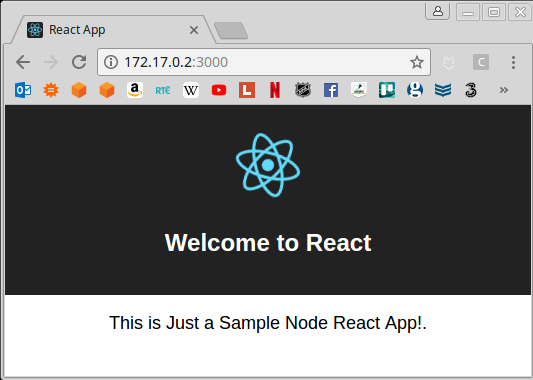
\includegraphics[width=\textwidth,keepaspectratio]{app-local}
		\label{fig:app-local}
	\end{figure}
	In order to implement continuous integration, the app will be built by means of a Docker image which can be pushed to a Docker Hub registry. True continous integration would often also implements testing before building the image\citep{docker}. However, as this is just a basic sample app not tests are included.
	
	To \textit{dockerise} the image a \textit{Dockerfile} was added to the source code. This \textit{Dockerfile} specifies a base image for the file (a standard node image for Docker Hub) and copies the source code into the image. It installs the necessary software (npm) and starts the app. It is worth noting that this is starting the app in development mode as opposed to building the app with \textit{npm build} as this is just for demonstration purposes. The \textit{Dockerfile} also exposes port 3000 of the container. This is the port on which the app run in development mode and can be observed in \autoref{fig:app-local}. Later, when the image is run on an ECS instance, this containers port will need to me mapped to a host port on the instance.
	
	\begin{minipage}{\textwidth}
		\begin{lstlisting}[caption={Dockerfile}]
			FROM node:carbon
			WORKDIR /usr/src/app
			COPY package*.json ./
			RUN npm install
			COPY . .
			EXPOSE 3000
			CMD ["npm", "start"]
		\end{lstlisting}
	\end{minipage}
	
	\subsection{Initial ECS setup}
	Some initial setup of ECS infrastructure was needed before the Jenkins job could run. This comprised of the following AWS services:
	
	\medbreak
	
	\noindent \textbf{ECS Cluster:}  An ECS cluster is a grouping of ECS instances. It allows scaling and load balancing of service such as a web app running in containers on multiple instances. As part this paper, autoscaling and load balancing are not implemented, however, they could be easily added by configuring a an Application Load Balancer and configuring the ECS Service to autoscale on some configured Cloudwatch alarms. This is not necessary however for the demonstration purposes of this paper. However, an ECS cluster must still be created, with the instance running the app registered to it.
	
	\begin{minipage}{\textwidth}
		\begin{lstlisting}[caption={Create ECS Cluster},language=bash]
		aws ecs create-cluster --cluster-name $CLUSTER_NAME
		\end{lstlisting}
	\end{minipage}
	
	\noindent \textbf{EC2 Instance:} This is where the app runs, albeit within a container. The instance must be an ECS optimised instance. This means is includes the ECS agent, a tool which runs on the instance allowing it to register with the cluster \citep{aws-agent}. It is registers with the cluster by way of user data.
	
	\begin{minipage}{\textwidth}
		\begin{lstlisting}[caption={Create EC2 Instance},label={create-instance},language=bash]
		aws ec2 run-instances --image-id $AMI_ID --count 1 --instance-type t2.micro --key-name $KEY_NAME --security-groups $HTTPSSH_SEC_GROUP $HTTP_GITHUB --iam-instance-profile Name=$ECS_INSTANCE_ROLE --user-data file://user-data --tag-specifications 'ResourceType=instance,Tags=[{Key=Name,Value='$INSTANCE_NAME'}]'
		\end{lstlisting}
	\end{minipage}
	
	\begin{minipage}{\textwidth}
		\begin{lstlisting}[caption={User Data},language=bash]
		#!/bin/bash	
		echo ECS_CLUSTER=node-app-cluster >> /etc/ecs/ecs.config	
		\end{lstlisting}
	\end{minipage}
	
	Notice in \autoref{create-instance} that the instance is configured with the EC2 Instance IAM role. In order for the ECS agent running on the instance to communicate with ECS via an API and register with the cluster, the instance needs permissions. By assigning this IAM role to the instance, it is able to assume this role. The role is granted permissions that allow it to issues commands to ECS such the necessary \textit{Register Container Instance}.
	
	\medbreak
	\noindent \textbf{Task Definition:}	The task definition contains instructions on running the app. For example, the image to use and from where to pull it. In this case, the image is pulled from a registry on Docker Hub.
	
	\begin{minipage}{\textwidth}
		\begin{lstlisting}[caption={Task Definition Template},label=task-def]
		{
			"family": "node-app",
			"volumes": [
				{
				"name": "my-vol",
				"host": {}
				}
			],
			"containerDefinitions": [
				{
					"environment": [],
					"name": "node-app",
					"image": "rshelly/sample-node-app:v_%BUILD_NUMBER%",
					"cpu": 10,
					"memory": 500,
					"portMappings": [
						{
							"containerPort": 3000,
							"hostPort": 80
						}
					],
					"mountPoints": [
						{
							"sourceVolume": "my-vol",
							"containerPath": "/var/www/my-vol"
						}
					],
					"essential": true
				}
			]
		}	
		\end{lstlisting}
	\end{minipage}
	
	Notice in \autoref{task-def} the build number parameter specified as the tag for the image. This is used because every time the Jenkins job runs, building the latest image, it will tag it with a version number (i.e. the build number). The task definition must specify that this latest image is to be used. Therefore, this task definition serves as a template for the Jenkins job to create up-to-date definitions every time a new image it built. For this reason, this task definition template was also placed on the Jenkins server where the job will have access to it.
	
	Also specified in the task definition is the port mappings. The container port is configured as port 3000 as this is the port on which the \textit{Dockerfile}, created above, exposes the app. This is mapped directly to host port 80, as not scaling is being implemented.
	
	As the Jenkins job has not run yet, there is no image in the registry yet. A dummy task definition with a build number of zero was registered with the cluster during the initial build.
	
	\begin{minipage}{\textwidth}
		\begin{lstlisting}[caption={Register Task Definition},language=bash]
		sed -e "s;%BUILD_NUMBER%;0;g" ./node-app.json > ./node-app-v_0.json
		aws ecs register-task-definition --cli-input-json file://node-app-v_0.json	
		\end{lstlisting}
	\end{minipage}
	
	\noindent \textbf{Service:} An ECS service runs the task definitions. It also takes care of scaling and load balancing. If these were implement it would have been a simple addtion to the service of adding the Applcation Autoscaling Policy and registering a Target Group for the instance(s).
	
	Every time a new image is built, Jenkins creates a new task definition to run the newly image from the Docker Hub registry. It then updates the service to run the new task definition in place of the old one. Therefore, the service must be created on ECS before the first run of the job. However, because no images have been built yet, it is configured with a desired count of zero. I.e. it will not run any task definitions.
	
	\begin{minipage}{\textwidth}
		\begin{lstlisting}[caption={Create Service},language=bash]
		aws ecs create-service --cluster $CLUSTER_NAME --service-name node-app-service --task-definition node-app --desired-count 0
		\end{lstlisting}
	\end{minipage}
		
	\subsection{Jenkins Setup}
	The Jenkins server was deployed to an AWS instance. The process of creating the Jenkins server was automated through two scripts. The first script is a python script with uses the Boto3 library to create and configure the necessary AWS infrastructure i.e. security groups and the instance. Note that during later development, more security groups were added to the instance. Due to size this script is not included as an appendix but can be viewed at the Github (see appendix \autoref{repos}).
	
	The second script is shown in appendix \autoref{install-jenkins}. This script installs Jenkins and Nginx to serve the Jenkins web console. It also install Docker and as it will be needed to build the image of the web app. As indicated above, the task definition templates was also added to the \textit{app} folder in the home directory where the Jenkins job can access it. Note that in practice this script was not run, but rather the commands were run on the instance via SSH.


	\subsection{Jenkins Job}
	Setting up the Jenkins job,
	\subsubsection{Credentials}
	maybe talk about the credentials plugin here and how credentials for AWS, dockerhub are managed
	\section{Running the Job}
	Just show that it works on git push